\documentclass[11pt,a4paper]{article}
\author{Michael James, 390198}

\usepackage[left=20mm,right=20mm,top=20mm,bottom=20mm]{geometry}
\usepackage[pdftex]{graphicx}
\usepackage[hyphens]{url}

\begin{document}

\title{Project 1: Approximate String Search for Geolocation of Tweets}
\maketitle

\section{Introduction}

The objective of Project 1 was to identify location names (ASCII strings) present within the body of a Tweet (an ASCII string between 1 and 140 characters in length). Edit distance matching techniques, including Variants of Global Edit Distance (Needleman-Wunsch) and Local Edit Distance (Smith-Waterman) matching algorithms, were explored in Project 1. 

\section{Preprocessing Input Data}  

Several heuristics were employed in the preprocessing of the tweets and locations input files to improve the performance of the string approximation algorithms explored in Project 1.\\\\
The reduction in the size of the input tweet and locations files, due to the preprocessing steps outlined below, are summarised in Table \ref{table:input-table}.

\subsection{Lowercase Input and Removal of Non-Alphabetic Characters (Excluding Space)}
\label{subsec:alpha}

To reduce the sample space, as specified as a requirement of the project specification, all non-alphabetic characters, excluding space, were removed from the body of the tweets. Additionally, all alphabetic characters within a tweet were made lower case. After this stage of tweet preprocessing it would have been impossible for a location name with non-alphabetic characters and/or uppercase letters to match a substring within any tweet bodies. Therefore, non-alphabetic characters were removed from the locations list and the alphabetic characters within the locations list were made lower case to ensure the location names remained consistent with the modified tweet bodies.

\subsection{Word Stemming}

Stemming is the process of reducing inflicted words to their stem (base form).A Porter Stemmer algorithm was used in the preprocessing of the location and tweet files. \\\\
The Porter Stemmer algorithm was found to further distort a subset of misspelled words within the tweet bodies, however the Porter Stemmer was also capable of (partially) correcting miss-spelled location words. Further, the Porter Stemmer reduced the sample space of the problem by introducing consistency in tweet words referring to the same location and reducing the number of characters in both the preprocessed tweet and location files.\\\\
A sample of differences between tweet and location strings with and without the Porter Stemmer preprocessing step can be seen in Tables \ref{table:stem-tweet} and \ref{table:stem-location}.
   
\begin{table} [h]
\caption{Stemming Tweets}
\begin{center}
	\begin{tabular}{| c | p{5.5cm} | p{5.5cm} |}
	\hline
	  & \multicolumn{2}{|c|}{\textbf{Tweet Text}}\\
	\hline
	\textbf{No Porter Stemming} &  hanh khangs wedding friends going fabulous night & foursquare made breakfast meeting morning bit interesting usual\\
	\hline
	\textbf{Porter Stemming}  & hanh khang wed friend fabul night & whi foursquar made breakfast meet thi morn bit interest usual\\
	\hline
	\end{tabular}
\end{center}
\label{table:stem-tweet}
\end{table}

\begin{table} [h]
\caption{Stemming Locations}
\begin{center}
	\begin{tabular}{| c | c | c | c | }
	\hline
	 &  \multicolumn{3}{|c|}{\textbf{Location Text}}\\
	\hline
	\textbf{No Porter Stemming} & aaa advanced air ambulance
& miami lakes & new york\\
	\hline
	\textbf{Porter Stemming} &  aaa advanc air ambul
& miami lake & new york\\
	\hline
	\end{tabular}
\end{center}
\label{table:stem-location}
\end{table}

\subsection{Removal of Stop Words And Excess White Space}
A large amount of tweets and locations contained words which were less than 3 characters in length and words which were extremely common in the English language (especially after preprocessing stage \ref{subsec:alpha}). Common words and words of one to two characters of length carried little entropy when determining whether the Twitter user was Tweeting about a location or using the words in another context (Table \ref{table:stop-words}).\\\\
Words of one-two characters and common words were removed from both the tweets and the locations list to further reduce processing time and avoid false positives. The list of stop words, contained within the NLPK library for python, was used to remove stop words from he locations and tweet texts.\\\\
It is worth noting that stop words can cause problems when searching for phrases (location names) that include them. However, after examination of the location and tweet files it was determined that the benefits of removing stop words outweighed the destruction of an insignificant amount of location names. 

\begin{table}[h]
	\centering
	\caption{Undesirable Location Name Matches Before Stop Word Removal (Smith-Waterman and Sub-Distance Algorithms)}
	\begin{tabular}{| l | p{10cm} |}
	\hline
	 \textbf{Matched Location Names} & \textbf{Matched Tweet}\\
	\hline
	's', 'm', 'th' & oooo thi man on schofe  s the cube isnt do too well is he\\
	\hline
	'b', 'l', 'y', 'm'  & dont get discourag with your busi i can helpw work as a team contact me at lsivagedynamicincomesolutionsorg\\
	\hline
	\end{tabular}
	\label{table:stop-words}
\end{table}

\subsection{Removal of Similar Locations}
After thorough inspection of the locations file, significant overlap between the start of many location strings could be seen. To further reduce the sample size of locations, locations which had their first two words or more in common were combined into one location containing the common substring (Table \ref{table:similar-locals}). The reduction in location sample space was traded off against the loss of the ability to match very specific locations.

\begin{table}[h]
\caption{Removal of Similar Location Names}	
\centering
	\begin{tabular}{| p{7cm} | p{7cm} | }
	\hline
	\textbf{Before Removal of Similar Locations} & \textbf{After Removal Of Similar Locations}\\
	\hline
	abid savior, abid savior commun church, abid savior evangel lutheran church, abid savior free lutheran church, abid savior lutheran church, abid savior lutheran church school, abid savior school & abid savior
	\\
	\hline
	\end{tabular}
\label{table:similar-locals}

\end{table}

\subsection{Removal of Duplicate Locations}       
After performing the preceding preprocessing steps, the locations list contained various duplicate entries. The duplicate locations were removed to avoid unnecessary processing of said duplicates.

\begin{table} [th]
\caption{Input Data Size Reduction}
\centering
	\begin{tabular}{| c | c | c |}
	\hline
	 &  \textbf{Word Count} & \textbf{Number of Locations}\\
	\hline
	\textbf{Raw Locations Input File} & 6,147,265 & 2,153,222\\
	\hline
	\textbf{Final Locations Input File} & 2,107,408 & 834,250\\
	\hline
	 &  & \\
	\hline
	\textbf{Raw Tweets Input File} & 66,491,876 & N/A\\
	\hline
	\textbf{Final Tweets Input File} & 37,143,754 & N/A\\
	\hline
	\end{tabular}
\label{table:input-table}
\end{table}

\section{Approximate String Matching Algorithms And Results}

\subsection{Needleman-Wunsch: Global Edit Distance Baselines}

\textbf{Needleman-Wunsch}, N-W, is a popular dynamic programming algorithm for calculating the edit distance between two strings. An edit distance is a metric for quantifying how dissimilar two strings are to one another. Edit distance functions associate a cost value with the basic operations of insertion, deletion, replacement and matching of characters required for conversion of one string into another string. The N-W algorithms implemented in project 1 used a \textbf{Levenshtein Distance} cost function to assign a cost of 1 for insertions, deletions and replacements and a cost of 0 for matches.\\\\
Two naive variants of N-W algorithms were established as algorithm baselines. The N-W baselines were used to allow us to determine the intrinsic difficulty of the Project 1 task and allow us to gauge the performance of other proposed solutions.

\subsubsection{N-W Whole String Comparison Baseline}

The first baseline method of N-W implementation involved comparing the whole body of tweet text against a location.\\\\
The run time of the N-W Whole String algorithm was extremely fast, with an average processing time of 2.884 seconds per tweet (see Figure \ref{fig:times-graph} for comparison of algorithm run times). The algorithmic complexity of the N-W Whole String algorithm is $O(nm)$ where n is the length of a location and m is the character length of a tweet. \\\\ 
This naive solution yielded poor matching results (Table \ref{table:alg-table1} and \ref{table:alg-table2}). The poor results can be attributed to the significant difference in the location and tweet lengths. The significant disparity between many location and tweet lengths resulted in a large number of deletions required for conversion of a tweet to a location, thus an unacceptably high Levenshtein difference for tweets which had location names surrounded by other words. Reducing the required threshold score for a location to be considered a match did not alleviate the poor performance, as the algorithm would then return an unacceptable amount of false positives.\\\\
The N-W Whole String Comparison algorithm provided an excellent runtime baseline as a goal.

% insert tables and figures supporting argument and maths


\subsubsection{N-W Tokenised Words Comparison Baseline}

To avoid the problems associated with comparing location and tweet bodies of vastly different lengths the location queries and tweet bodies were tokenised into words. A location containing N words was compared with all tweet sub-strings containing N words.\\\\
This brutforce style algorithm had better matching capabilities as seen in the tweet exerts of Table \ref{table:alg-table1} and \ref{table:alg-table2}. However, the running time of N-W Word Tokens was significantly larger, with an average run time of 17.49 seconds per tweet (Figure \ref{fig:times-graph}).\\\\
The N-W Tokenised Words Comparison provided excellent location-tweet matching baseline goal.

% Add tables and table references and mathamatical analysis

\subsection{Smith-Waterman: Local Edit Distance}

The Smith-Waterman (S-W) algorithm finds the maximum length of the substring in common between two strings. S-W was considered as a candidate solution due to exhibiting the same complexity as N-W Whole String Comparison, $O(nm)$, combined with the potential for the better location-tweet matching, associated with the Tokenised N-W baseline, due to  S-W ignoring the disparity in length between a tweet and location.\\\\
A score of 1 was assigned for a match and -1 for a deletion, insertion and replacement. The S-W match threshold was normalised by dividing the length of the matching substring by the minimum length of the location string compared to the tweet string. A threshold score greater than or equal to 0.90 was considered to be a match (as determined by subjective human judgement).\\\\
The S-W algorithm produced a runtime of 3.942 seconds. The S-W closely approximated the N-W Whole String baseline runtime (Figure \ref{fig:times-graph}).\\\\      
The S-W closely matched the goal matching baseline of the N-W tokenised words algorithm (Table \ref{table:alg-table1} and \ref{table:alg-table2}). However, often S-W would return more matches than N-W tokenised words, as S-W would NOT penalise location words which started mid-word in the tweet text. The additional matches returned by S-W were often considered inappropriate as they were often sub-words contained within bigger words. For example, the location 'ash' was returned by the S-W and not by N-W tokenised words, as S-W had found a match within the word 'washington'.    

\subsection{Sub-Distance: Needlemen-Wunsch and Smith-Waterman Combined}

The runtime and matching of the Smith-Waterman was a definite step forward in finding an edit-distance based solution to the string approximation task of Project 1. However, the disadvantage of location strings being matched anywhere within the longer tweet string, including mid-word, without penalty resulted in additional false positives. The Sub-Distance algorithm was developed to address this S-W undesirable characteristic.\\\\
Sub-Distance involved implementing two small changes to the N-W whole string matching algorithm:
\begin{itemize}
\item The initialisation of the row associated with the empty character in the location name and the tweet text was altered to have an edit distance score associated with the depth of a character in a word NOT the whole string (Table \ref{table:subdist}). The intuition behind this change is that location matches that start on empty space or a word should not be penalised, however location matches that start mid-word should be penalised in relation to how deep into the word said match is.
\item Once the scores of the bottom row had been calculated, the lowest score was taken as the edit-distance cost, rather than the score in the rightmost corner. This effectively meant that we didn't care how many characters we skipped after we stopped matching. 
\end{itemize}
Sub-Distance has a slightly smaller runtime than S-W and N-W Whole String, 2.83 seconds. Sub-Distances runtime result was expected as both N-W whole string and S-W have the same complexity as Sub-Distance, $O(nm)$.\\\\
Sub-Distance achieved closer matching to the N-W Tokenised Words baseline than S-W (Table \ref{table:alg-table1} and \ref{table:alg-table2}). However, Sub-Distance generated more false-positives than N-W Tokenised Words, as Sub-Distance still suffered from not penalising location matches that matched the prefix of a larger word (similar to S-W).

\begin{table}[ht]
	\centering
	\caption{Sub-Distance Edit Distance Matrix Initialisation}
    \begin{tabular}{l|lllllllllllllllll}
    ~ & ~ & m & i & a & m & i & ~ & v & i & c & e & ~ & m & o & v & i & e \\
    \hline
    ~ & 0 & 1 & 2 & 3 & 4 & 5 & 0 & 1 & 2 & 3 & 4 & 0 & 1 & 2 & 3 & 4 & 5 \\
    m & 1 & ~ & ~ & ~ & ~ & ~ & ~ & ~ & ~ & ~ & ~ & ~ & ~ & ~ & ~ & ~ & ~ \\
    i & 2 & ~ & ~ & ~ & ~ & ~ & ~ & ~ & ~ & ~ & ~ & ~ & ~ & ~ & ~ & ~ & ~ \\
    a & 3 & ~ & ~ & ~ & ~ & ~ & ~ & ~ & ~ & ~ & ~ & ~ & ~ & ~ & ~ & ~ & ~ \\
    m & 4 & ~ & ~ & ~ & ~ & ~ & ~ & ~ & ~ & ~ & ~ & ~ & ~ & ~ & ~ & ~ & ~ \\
    i & 5 & ~ & ~ & ~ & ~ & ~ & ~ & ~ & ~ & ~ & ~ & ~ & ~ & ~ & ~ & ~ & ~ \\
    \end{tabular}
    \label{table:subdist}
\end{table}


\section{Conclusion}

Four methods were considered for string approximation of location names that reside within tweet bodies. Pure N-W suffered in matching performance due to the large disparity in matching string sizes. Tokenised N-W returned the most suitable matches, however suffered from an extremely long processing time. S-W found the middle ground between pure N-W and Tokenised N-W, providing location matching from within a tweet with a better runtime, however returned more false positives due to matching location names within words. Sub-Distance, employed clever initialisation and exit parameters to Pure N-W to achieve better matching than S-W with the same complexity.\\\\
The shortest runtime for a single tweet to be compared to all queries was 2.8 seconds (Sub-Distance). Therefore, to process all 3.6 million preprocessed tweets against all of the preprocessed locations would take over 116 days. If the whole Location-Tweet sample space had to be analysed faster methods of string approximation, such as the use of Tries or N-gram matching algorithms, are an area for further research. 

\begin{figure}[ht]
	\centering
	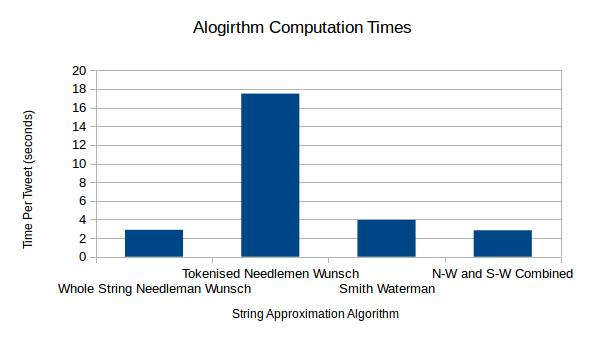
\includegraphics[scale=0.8]{times1.jpg}
	\label{fig:times-graph}
	\caption{Comparison of Algorithm Run Times For A Given Tweet Compared To All Of the Location Queries (over a sample of 1000 Tweets for Tokenised N-W and a sample of 10000 Tweets For The Remaining Algorithms)}
\end{figure}

\begin{table} [t]
\caption{Sample Tweet And Matches}
\begin{center}
	\begin{tabular}{| p{5.5cm} | p{10cm} |}
	\hline
	\multicolumn{2}{|p{15.5cm}|}{\textbf{Tweet Text:} washington folk gap reopen tyson acoust set come } \\
	\hline
	\textbf{Algorithm} & \textbf{Match-Score Pairs}\\
	\hline
	Baseline Needlemen-Wunsch & \\
	\hline
	Brutforce Needlemen-Wunsch & ('folk', 100), ('gap', 100), ('tyson', 100), ('washington', 100), ('washington fork', 93), ('washington oak', 90)]\\
	\hline
	Waterman-Smith & ('ash', 1.0), ('cous', 1.0), ('folk', 1.0), ('gap', 1.0), ('open', 1.0), ('pen', 1.0), ('reo', 1.0), ('tyson', 1.0), ('wash', 1.0), ('washington', 1.0)]\\
	\hline
	N-W and S-W Combined & ('folk', 1.0), ('gap', 1.0), ('reo', 1.0), ('tyson', 1.0), ('wash', 1.0), ('washington', 1.0), ('washington fork', 0.933)\\
	\hline
	\end{tabular}
\end{center}
\label{table:alg-table1}
\end{table}

\begin{table} [t]
\caption{Sample Tweet And Matches}
\begin{center}
	\begin{tabular}{| p{5.5cm} | p{10cm} |}
	\hline
	\multicolumn{2}{|p{15.5cm}|}{\textbf{Tweet Text:} american red cross blood drive moffat build ampm welcom check detail httpbitlyqtpp
} \\
	\hline
	\textbf{Algorithm} & \textbf{Match-Score Pairs}\\
	\hline
	Baseline Needlemen-Wunsch & \\
	\hline
	Brutforce Needlemen-Wunsch & ('america', 93), ('american', 100), ('american red cross', 100), ('americana', 94), ('blood river', 91), ('build', 100), ('check', 100), ('cross', 100), ('driver', 91), ('mcross', 91), ('moffat', 100), ('moffatt', 92), ('readi cross', 90), ('red', 100), ('red cross', 100), ('reed cross', 95), ('ucross', 91), ('welcom', 100)\\
	\hline
	Waterman-Smith & ('ame', 1.0), ('ameri', 1.0), ('america', 1.0), ('american', 1.0), ('american red cross', 1.0), ('build', 1.0), ('check', 1.0), ('cross', 1.0), ('elco', 1.0), ('eri', 1.0), ('erica', 1.0), ('fat build', 1.0), ('heck', 1.0), ('ive', 1.0), ('mer', 1.0), ('moffat', 1.0), ('red', 1.0), ('red cross', 1.0), ('rive', 1.0), ('ross', 1.0), ('tail', 1.0), ('welcom', 1.0)]\\
	\hline
	N-W and S-W Combined & ('ame', 1.0), ('ameri', 1.0), ('america', 1.0), ('american', 1.0), ('american red cross', 1.0), ('build', 1.0), ('check', 1.0), ('cross', 1.0), ('moffat', 1.0), ('red', 1.0), ('red cross', 1.0), ('reed cross', 0.9), ('welcom', 1.0)\\
	\hline
	\end{tabular}
\end{center}
\label{table:alg-table2}
\end{table}

\begin{thebibliography}{9}

\bibitem{lamport94}
  Leslie Lamport,
  \emph{\LaTeX: a document preparation system}.
  Addison Wesley, Massachusetts,
  2nd edition,
  1994.

\end{thebibliography}

\end{document}